\documentclass[tikz, margin=2mm]{standalone}
\usetikzlibrary {lindenmayersystems}
\begin{document}
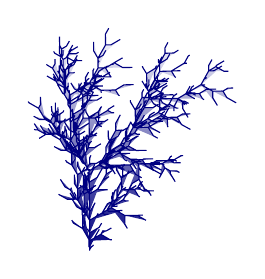
\begin{tikzpicture}
%\draw [green!50!black, rotate=90]
\shadedraw [top color=white, bottom color=blue!50!black, draw=blue!50!black, rotate=90]
  [l-system={rule set={F -> FF-[-F+F]+[+F-F]}, axiom=F, order=4, step=2pt,
     randomize step percent=40, angle=30, randomize angle percent=3}]
       lindenmayer system;
\end{tikzpicture}
\end{document}
